\documentclass[twoside]{report}

\usepackage{color}
\usepackage{amsmath,amsfonts}
\usepackage{graphicx}

\usepackage[pdftex,hypertexnames=false,
            colorlinks=true,
            pdfstartview=FitV,
            linkcolor=black,
            citecolor=black,
            urlcolor=black,
            pdfpagelabels,
            naturalnames=true]{hyperref}

\newcommand\myurl[2]{\url{#1}} % Strip periods after URLs

\newcommand{\red}[1]{{\color{red} #1}}
\newcommand{\todo}[1]{\textbf{TODO: #1}}

\newcommand{\software}[1]{\texttt{#1}}
\newcommand{\libMesh}{\software{libMesh}}
\newcommand{\GRINS}{\software{GRINS}}
\newcommand{\FEMSystem}{\software{FEMSystem}}

\newcommand{\bx}{\boldsymbol{x}}
\newcommand{\bu}{\boldsymbol{u}}
\newcommand{\bv}{\boldsymbol{v}}
\newcommand{\bn}{\boldsymbol{n}}
\newcommand{\bg}{\boldsymbol{g}}
\newcommand{\bI}{\boldsymbol{I}}


\begin{document}

\author{Paul T. Bauman \and Roy H. Stogner}
\title{GRINS Multiphysics Framework:\\
Theory Documentation}
\maketitle
\tableofcontents

\chapter{Notation}
We will generally be discussing weak formulation of PDEs on open
connected subsets of $\mathbb{R}^n$, $n$ = 1, 2, or 3, denoted
$\Omega$. We denote the boundary of $\Omega$ as $\Gamma$. $\Gamma$ can
be partitioned in many ways, but typically we consider $\Gamma_D$, the
part of $\Gamma$ where Dirichlet boundary conditions are imposed and
$\Gamma_N$ where Neumann conditions are applied. For systems with
multiple unknown variables, we can partition the boundary $\Gamma$
differently for each variable. We'll append the variable name to the
subscript, e.g. the Neumann part of the boundary for the velocity
variable $\bu$ will be denoted at $\Gamma_{N,\bu}$.

We use typical inner product notation for integrals over $\Omega$:
%
\begin{equation}
\left( \bu, \bv \right) := \int_{\Omega} \bu \cdot \bv \; d\bx
\end{equation}
%


\chapter{Boussinesq Buoyancy}

\chapter{Elastic Cable}

\chapter{Elastic Membrane}

\chapter{Convective Heat Transfer}

\chapter{Incompressible Navier-Stokes}

\chapter{Incompressible Navier-Stokes Stabilization}
\section{``Adjoint'' Stabilization}
\section{``SPGSM'' Stabilization}

\chapter{Low Mach Navier-Stokes}
\subsection{Background Information}
The derivation detailed herein is for computing analytical Jacobians for the Low Mach Navier-Stokes equations. The final results are then implemented in GRINS src/physics/src/low\_mach\_navier\_stokes.C, with the goal being that there
will be a significant speedup in computation over using the standard finite difference approximation. The derivation is broken up into 3 subsections: mass (P residual), momentum (U residual), and energy (T residual).
Note that a sign convention has been specified for purposes of optimization.\\
Also note that, in this case, the following parameters are considered functions of temperature, T:
\begin{itemize}
    \item density, $\rho$
    \item specific heat, $c_p$
    \item viscosity, $\mu$
    \item thermal conductivity, $k$
\end{itemize}
For the formulations, \textbf{u}=\{$P,U,T$\} and the test functions \textbf{$\Phi$}=\{$\xi,\phi,\psi$\}.\\
The variable names used in the code follow this template: $Kxy$, where $x$ is the residual and $y$ is the derivation variable.  For example, $KPT$ is the derivative of the P residual with respect to temperature,
while $KuP$ is the derivative of the $u$-velocity component of the U residual with respect to pressure. \newline
Lastly, a note on notation. Index notation is used throughout this section in order to make the derivations clearer. Indices $a-h$ are used for vector components, while $i-r$ are used for degrees of freedom.
Also note that Cartesian coordiantes are assumed for these derivations. As such, in the momentum equation in particular, terms of the following form may appear: $\phi_i^{a,b}$. In the index notation used herein for the case
where both sub- and superscripts appear on a single variable, 
subscripts refer exclusively to degrees of freedom, while superscripts are used exclusively for vector operations (i.e. divergence or gradient).

\newpage
%%%%%%%%%%%%%%%%%%%%%%%%%%%%%%%%%%%%%%%%%%%%%%%%
\subsection{Mass Equation}
The given P residual:
\begin{equation}
    F_{p,i} = (-(U \cdot \nabla T) T^{-1} + \nabla \cdot U)\xi_i
\end{equation}

Now converting to tensor notation

\begin{equation}
    F_{p,i} = -u_a T_{,a} T^{-1} \xi_i + u_{b,b}\xi_i
\end{equation}

Galerkin approximation:
\begin{align*}
    u_a &= \sum_i u_i \phi_i^a\\
    T &= \sum_i T_i \psi_i
\end{align*}

\begin{equation}
    F_{p,i} = -u_k \phi_k^a T_l \psi_l^{,a} (T_m \psi_m)^{-1} \xi_i + u_n \phi_n^{b,b} \xi_i
\end{equation}

The P residual is a function of velocity, $U$, and temperature, $T$, so derivatives must be taken with respect to both of them using the following form:

\begin{align*}
    \frac{\partial}{\partial u_j} (u_i \phi_i^a) &= \phi_j^a \\
    \frac{\partial}{\partial T_j} (T_i \psi_i) &= \psi_j
\end{align*}

\begin{align}
    \frac{\partial F_{p,i}}{\partial u_j} = &-\phi_j^{a} T_l \psi_l^{,a} (T_m \psi_m)^{-1} \xi_i + \phi_j^{b,b} \xi_i \nonumber \\
    \frac{\partial F_{p,i}}{\partial u_j} = &-\phi_j^{a} T_{,a} T^{-1} \xi_i + \phi_j^{b,b} \xi_i \label {fp_du}\\ 
    \nonumber \\
    \frac{\partial F_{p,i}}{\partial T_j} = &-u_k \phi_k^a \xi_i \left [ T_l
\psi_l^{,c} (-1) (T_m \psi_m)^{-2} (\psi_j) + (T_n \psi_n)^{-1} \psi_j^{,d} \right ] + 0 \nonumber \\
    \frac{\partial F_{p,i}}{\partial T_j} = &u_c T_{,c} T^{-2} \psi_j \xi_i - u_d T^{-1} \psi_j^{,d} \xi_i \label{fp_dT}
\end{align}

Equations \ref{fp_du} and \ref{fp_dT} above are the generalized Jacobian terms for the P residual. When implemented in LMNS.C, the following terms will result:\\
$KPu, KPv, KPw, KPT$

\newpage
%%%%%%%%%%%%%%%%%%%%%%%%%%%%%%%%%%%%%%%%%%%%%%%%%%%%%%
\subsection{Momentum Equation}
The U residual is given in vector and tensor notation as follows:
\begin{align}
    F_{U,i} &= -\rho u \cdot \nabla u \cdot \phi_i + P(\nabla \cdot \phi_i) - \mu \left [\nabla u : \nabla \phi_i + (\nabla u)^T : \nabla \phi_i - \frac{2}{3} (\nabla \cdot u) I : \nabla \phi_i \right ] + \rho \mathbf{g} \cdot \phi_i \\
    F_{U,i}^a &= -\rho u_b u_{a,b} \phi_i^a + P\phi_i^{a,a} - \mu \left [u_{a,c} \phi_i^{a,c} + u_{d,a} \phi_i^{a,d} - \frac{2}{3} u_{e,e} \delta_{a,f} \phi_i^{a,f} \right ] + \rho g_a \phi_i^a \ (no \ sum \ on \ a) \label{Fui_tensor}
\end{align}

Note that in \ref{Fui_tensor}, $\delta_{a,f}$ is the Kronecker delta function. \\

Now, the Galerkin approximation

\begin{align*}
    u_a &= \sum_i u_i \phi_i^a\\
    P &= \sum_i P_i \xi_i\\
    T &= \sum_i T_i \psi_i
\end{align*}

\begin{align}
    F_{U,i}^a =  -\rho u_k \phi_k^b u_l \phi_l^{a,b} \phi_i^a + P_m \xi_m \phi_i^{a,a} - \mu \left [u_n \phi_n^{a,c} \phi_i^{a,c} + u_o \phi_o^{d,a} \phi_i^{a,d} - \frac{2}{3} u_p \phi_p^{e,e} \delta_{a,f} \phi_i^{a,f} \right ] + \rho g_a \phi_i^a \label{u_resid}
\end{align}

Equation \ref{u_resid} above is a function of velocity, pressure, and temperature (due to $\rho = \rho(T)$ and $\mu = \mu(T)$ \ ), so derivatives must be taken with respect to all of them.\\
\textbf{Also note that, as stated in \ref{Fui_tensor}, there is no sum over index $a$}.

\begin{align}
   \frac{\partial F_{U,i}^a}{\partial u_j} = &-\rho \left [ u_k \phi_k^b \phi_j^{a,b} + u_l \phi_l^{a,g} \phi_j^g \right ] \phi_i^a 
        + 0 - \mu \left [\phi_j^{a,c} \phi_i^{a,c} + \phi_j^{d,a} \phi_i^{a,d} - \frac{2}{3} \phi_j^{e,e} \delta_{a,f} \phi_i^{a,f} \right ] \nonumber \\     
   \frac{\partial F_{U,i}^a}{\partial u_j} = &-\rho \left [ u_b \phi_j^{a,b} + u_{a,g} \phi_j^g \right ] \phi_i^a 
        - \mu \left [\phi_j^{a,c} \phi_i^{a,c} + \phi_j^{d,a} \phi_i^{a,d} - \frac{2}{3} \phi_j^{e,e} \delta_{a,f} \phi_i^{a,f} \right ] \label{du_du} \\
   \nonumber \\ 
   \frac{\partial F_{U,i}^a}{\partial P_j} = &\xi_j \phi^{a,a} \label{du_dp} \\
   \nonumber \\
   \frac{\partial F_{U,i}^a}{\partial T_j} = &-\frac{d\rho}{dT} \frac{d}{dT_j}(T_k \psi_k) u_l \phi_l^b u_m \phi_m^{a,b} \phi_i^a
        + 0 \nonumber \\ &- \left[ 0 + \frac{d\mu}{dT} \frac{d}{dT_j}(T_n \psi_n) [u_o \phi_o^{a,c} \phi_i^{a,c} + u_p \phi_p^{d,a} \phi_i^{a,d} - \frac{2}{3} u_q \phi_q^{e,e} \delta_{a,f} \phi_i^{a,f} ] \right ] \nonumber
        \\ &+ \frac{d\rho}{dT} \frac{d}{dT_m}(T_r \psi_r) g_a \phi_a \nonumber \\       
   \frac{\partial F_{U,i}^a}{\partial T_j} = &-\frac{d\rho}{dT} \psi_j u_b u_{a,b} \phi_i^a
        - \frac{d\mu}{dT} \psi_j \left [u_{a,c} \phi_i^{a,c} + u_{d,a} \phi_i^{a,d} - \frac{2}{3} u_{e,e} \delta_{a,f} \phi_i^{a,f} \right ]
        + \frac{d\rho}{dT} \psi_j g_a \phi_i^a \label{du_dT} 
\end{align}

Equations \ref{du_du}, \ref{du_dp}, and \ref{du_dT} above can then be implement in LMNS.C to create the following terms:\\
$Kuu, Kuv, Kuw, Kvu, Kvv, Kvw, Kwu, Kwv, Kww, KuT, KvT, KwT, KuP, KvP, KwP$

\newpage
%%%%%%%%%%%%%%%%%%%%%%%%%%%%%%%%%%%%%%%%%%%%%%%%%%%%%
\subsection{Energy Equation}
The T residual is given as follows:
\begin{align}
    F_{T,i} &= -\rho c_p (u \cdot \nabla T) \psi_i - k ( \nabla T \cdot \nabla \psi_i) \\
    F_{T,i} &= -\rho c_p (u_a T_{,a})\psi_i - k T_{,b} \psi_i^{,b}
\end{align}

Again, note that $\rho = \rho(T)$, $c_p = c_p(T)$, and $k = k(T)$

\begin{align}
    F_{T,i} = -\rho c_p u_k \phi_k^a T_l \psi_l^{,a} \psi_i - k T_m \psi_m^{,b} \psi_i^{,b}
\end{align}

Noting $F_{T,i}$ is a function of velocity and temperature.

\begin{align}
    \frac{\partial F_{T,i}}{\partial u_j} = &-\rho c_p \phi_j^a T_l \psi_l^{,a} \psi_i - 0 \nonumber \\
    \frac{\partial F_{T,i}}{\partial u_j} = &-\rho c_p \phi_j^a T_{,a} \psi_i \label{dT_du} \\
    \nonumber \\
    \frac{\partial F_{T,i}}{\partial T_j} = &-\psi_i \left [ \rho [ c_p u_k \phi_k^a \psi_j^{,a} + u_l \phi_l^b T_m \psi_m^{,b} \frac{d c_p}{dT} \psi_j ] + 
    [ c_p u_n \phi_n^{c} T_o \psi_o^{,c} ] \frac{d \rho}{dT} \psi_j  \right ] \nonumber \\
                                      &- k \psi_j^{,d} \psi_i^{,d} - T_p \psi_p^{,e} \psi_i^{,e} \frac{dk}{dT} \psi_j \nonumber \\
    \frac{\partial F_{T,i}}{\partial T_j} = &-\psi_i \left [ \rho [ c_p u_a \psi_j^{,a} + u_b T_{,b} \frac{d c_p}{dT} \psi_j ] + 
    [ c_p u_c T_{,c} ] \frac{d \rho}{dT} \psi_j  \right ] \nonumber \\
                                      &- k \psi_j^{,d} \psi_i^{,d} - T_{,e} \psi_i^{,e} \frac{dk}{dT} \psi_j \label{dT_dT}
\end{align}

Equations \ref{dT_du} and \ref{dT_dT} above will result in the following terms for LMNS.C:\\
$KTu, KTv, KTw, KTT$

\end{document}


\chapter{Low Mach Navier-Stokes Stabilization}
\section{``Adjoint'' Stabilization}
\section{``SPGSM'' Stabilization}

\chapter{Reacting Low Mach Navier-Stokes}

\chapter{Reacing Low Mach Navier-Stokes Stabilization}
\section{``Adjoint'' Stabilization}
\section{``SPGSM'' Stabilization}

\chapter{Penalty Method Representation}
\section{Turbine Definitions}

The normal in the blade's velocity direction is, 
\begin{equation}
n_B = \frac{u_B}{||u_B||}. 
\end{equation}
Where $u_B$ is the blade velocity and is specified.
The normal in the fan vertical direction is also set, and is typically, 
\begin{equation}
n_v = \left(0,0,1\right)
\end{equation}
e.g. pointing ``up''. Then the normal in the radial direction must be, 
\begin{equation}
n_r = n_B \times n_v. 
\end{equation}

Then, the fan-wing-plane component (e.g. the plane perpendicular to the 
radius) of local relative velocity is
\begin{equation}
u_p = u - (u\cdot n_r)\cdot n_r - u_B. 
\end{equation}
We can now define the lift and drag normals, where the direction
opposing drag is, 
\begin{equation}
n_{\text{drag}} = \frac{u_p}{||u_p||} 
\end{equation}
and the direction opposing lift orthogonal to the drag and the radial direction, 
\begin{equation}
n_{\text{lift}}= n_{\text{drag}} \times n_r. 
\end{equation}
Now the ``forward velocity'' in the reference frame of the turbine is, 
\begin{equation}
u_{\text{fwd}}= -u_p \cdot n_B
\end{equation}
and the ``upward'' velocity in this frame is, 
\begin{equation}
u_{\text{up}} = u_p \cdot n_v. 
\end{equation}
Finally, we can specify the angle with respect to the fan velocity
direction as, 
\begin{equation}
 \theta_f = \text{atan2}\left(\frac{u_{\text{up}}}{u_{\text{fwd}}}\right)
 %\theta_f = \text{tan}^{-1}\left(\frac{u_{\text{up}}}{u_{\text{fwd}}}\right)
\end{equation}
while the angle with respect to the chord is this with the addition of
the angle of attack of the blade, 
\begin{equation}
 \theta = \theta_f + \alpha(r).
\end{equation}
Now, we only need the drag polars in order to fully specify the force
on the blades.

\newpage
\section{Drag Polars}

Finally, continuous curves for coefficients of lift and drag 
must be specified. 
For the flat plate, the drag polars are specified as,

\begin{lstlisting}
    theta := ((t+pi/2)%pi)-pi/2; 
    lift   = 'if(abs(theta)<pi/24,theta*9,sin(2*theta))'
    drag   = 'if(abs(theta)<pi/24,0.005+theta*theta*81/25,1-0.8*cos(2*theta))'
\end{lstlisting}
for example. 

\begin{figure}[!htb]
  \begin{center}
    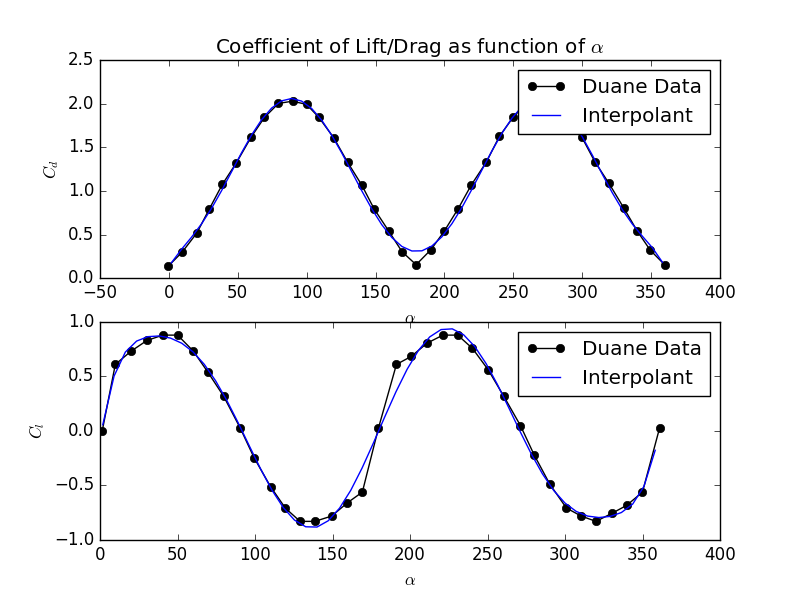
\includegraphics[width = 12 cm]{figs/flat}
    \caption{The flat plate interpolation.} 
    \label{flat}
  \end{center}
\end{figure}
As shown in Figure \ref{flat}, the fit is largely accurate to experimental data
as a point of comparison. 

At this point, we can calculate the force 
on the turbine as, 
\begin{equation}
 \boxed{F = \frac{1}{2}\frac{\rho u_p^2 C}{A}\left(C_l \cdot
					      n_\text{lift} + C_d \cdot n_\text{drag}  \right)}
\end{equation}

Where C is the chord length (specified as input), and A is the area,
which is also specified. For instance, the area swept might be, 
\begin{lstlisting}
     area_swept = '{r:=sqrt(x^2+y^2); 2*pi*r*(.6-.4)/4}'
\end{lstlisting}
for a 4 blade fan. The chord is specified similarly, for instance, 
\begin{lstlisting}
     chord_length = '.2*sqrt(2)'
\end{lstlisting}
would set a 0.28 meter chord length. 

Note that since GRINS is providing a volumetric forcing, 
the actual calculation will be of the form,

\begin{equation}
 \boxed{n F / 2 \pi r t = F'''}
\end{equation}
Where $t$ is the thickness of the turbine forcing region, and $n$ are the number of blades, 
or ''area swept``.

\bibliographystyle{abbrv}
\bibliography{refs}

\end{document}
